\section{Data Exploration and Preprocessing}
\label{section:expandpre}
The first step of this project consisted in a preliminary exploration of the dataset to better understand its characteristics.

The idea at the very base of this process is to take advantage of human abilities for selecting an appropriate preprocessing chain and looking for dirty data that should be cleaned or discarded. Moreover, we tried to take in consideration only useful attributes that best suit the assigned task.

To ease our job throughout all the process described in this report we decided to take advantage of the RapidMiner tool.

The initial dataset contains:
\begin{itemize}
\item \texttt{Probe}, which is the vehicle identifier;
\item \texttt{Cycle}, which identifies a period in which the engine vehicle is on;
\item \texttt{Transmission} and \texttt{RawData}, which are identifiers for the GSM connection and packets;
\item \texttt{Probe Date/Time}, which is the server time;
\item \texttt{GPS Date/Time}, which is the car time;
\item Vehicle \texttt{Speed} and \texttt{Acceleration};
\item \texttt{GPS Sat. Count}, which representes the number of satellites visibile to the GPS;
\item \texttt{GPS-0}, \texttt{GPS-1}, and \texttt{Altitude}, which are respectively Longitude, Latitude, and Altitude measured by the GPS system;
\item \texttt{GPS Speed}, which is the speed at which the vehicle is running according to the GPS;
\item \texttt{Eng. Speed}, \texttt{Eng. Load}, \texttt{Torque}, \texttt{Fuel Rate}, \texttt{CO2 Rate}, \texttt{Eng. Temp}, which are engine parameters.
\end{itemize}
We decided to take in consideration a subset of these attributes:
\begin{itemize}
\item \texttt{GPS Date/Time}, renamed to \texttt{GPSDate}, is used to simplify the time series;
\item \texttt{GPS-0, GPS-1}, which are used later in the mining process to find correlations between vehicle speed and geographical position;
\item \texttt{Speed}, which is smoothed with a simple moving average, then averaged with respect to the window applied to the time series and finally normalized;
\item \texttt{Eng. Speed}, renamed in \texttt{EngineSpeed}, which undergoes the same procedure described for the Speed attributes.
\end{itemize}
We decided not to take into account attributes like Acceleration, Torque, and Fuel Rate since they are - for real - strictly correlated to Speed and EngineSpeed and thanks to some mining test we notice that they don't have that much weight in the clustering operation.

Going deeper with the preprocessing phase we needed a work chain that is able to eliminate the noise due to the sampling of real data and all the attributes we didn't care about.
In Figure~\ref{figure:clean} is shown the very first tool-chain used to in the preprocessing phase.\newline


\begin{wrapfigure}{r}{0.4\textwidth}
  \begin{center}
    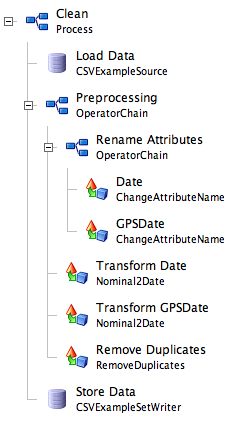
\includegraphics[scale=0.55]{images/clean.png}
  \end{center}
  \caption{Clean Process}
  \label{figure:clean}
\end{wrapfigure}


%\begin{figure}[h!]
%\centerline{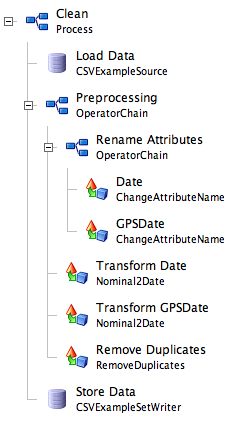
\includegraphics[scale=0.8]{images/clean.png}}
%\caption{Clean Process}
%\label{figure:clean}
%\end{figure}



First of all, we loaded the dataset thanks to an ad-hoc CSV\footnote{Comma Separated Values} reader operator, then we renamed date attributes and converted them in suitable format thanks to appropriate components. After these operations we removed duplicates based on the GPSDate attribute. This first phase ends with the component which is in charge of writing the resulting CSV dataset. These steps were necessary and repeated for every input dataset.\newline

After this cleaning process we needed to work on attributes in order to select only the meaningful ones and to elaborate some of them to have suitable values for clustering. This second tool-chain is represented in Figure~\ref{figure:preprocess}.

\begin{figure}[!]
\centerline{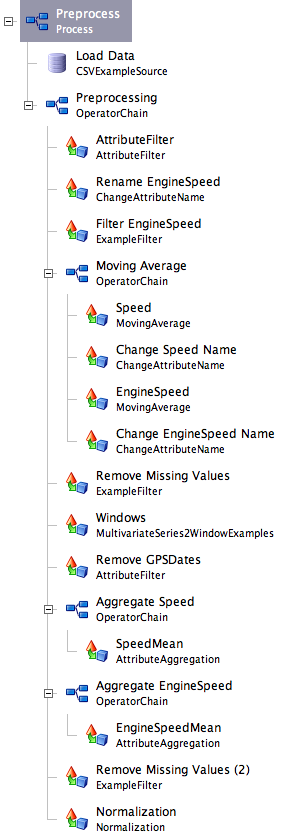
\includegraphics[scale=0.7]{images/preprocess.png}}
\caption{Preprocess}
\label{figure:preprocess}
\end{figure}

With this second work-flow we loaded a cleaned dataset on which we applied some attributes renaming and filter operators to select only a subset of attributes.
The real preprocessing step consisted in applying the moving average on the Speed and EngineSpeed attributes in order to smooth their values. Since the moving average works on a sliding set of values and some of these are missing, we needed to prune the corresponding instances from the dataset before proceeding with the operations.

